\section{SVM}

Máquinas de Vetores de Suporte, do inglês \textit{Support Vector Machines}, é um tipo de algoritmo de Aprendizado de Máquina supervisionado, utilizado para problemas de classificação envolvendo duas ou mais classes. O algoritmo foi proposto por \cite{Cortes:1995}. 

A ideia do SVM é mapear vetores de entrada em alguma dimensão maior, através de algum mapeamento não-linear, escolhido a piori. Neste novo espaço um hiperplano é construído para separar os dados \cite{Cortes:1995}.

\begin{figure}[ht!]
    \centering
    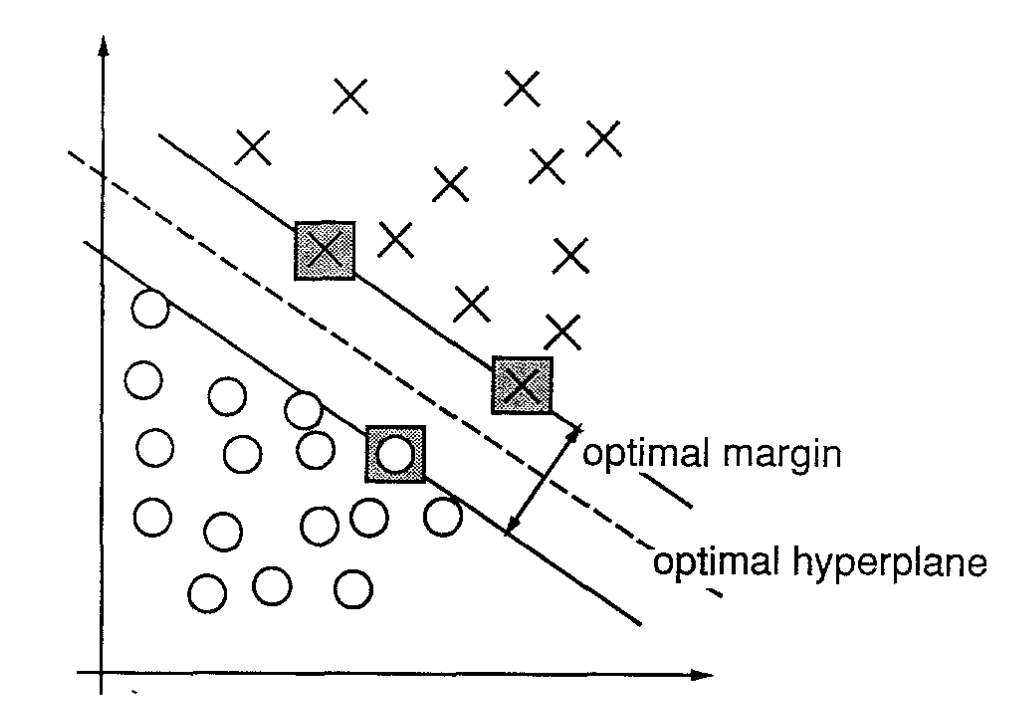
\includegraphics[scale=0.70]{Imagens/svm-exemplo.png}
    \caption{Um exemplo de um conjunto de dados linearmente separável em duas dimensões. \cite{Cortes:1995}}
    \label{fig:svm-exemplo}
\end{figure}

A figura \ref{fig:svm-exemplo} mostra um conjunto de dados que pode ser separado de maneira linear. O objetivo do SVM é encontrar o melhor hiperplano, de maneira que a margem\footnote{Margem é o dobro da distância entre o hiperplano e o ponto mais perto} seja a maior possível. 

\subsection{Vantagens e Desvantagens}
Um \textit{Support Vector Machine} é um modelo de classificação poderoso e versátil, capaz de realizar classificação linear e não linear, regressão e até detecção de \textit{outliers}. SVMs são parcularmente bem adequadas para problemas de classificação complexo, porém com \textit{datasets} não muito grandes \cite{Geron:2017}.

Um lado negativo do SVM é sua sensibilidade à escala dos dados de entrada. A figura \ref{fig:svm-escala} ilustra bem esse problema: no desenho da esquerda, aonde $x_0$ e $x_1$ estão em escalas diferentes, a margem é bem pequena. Quando os dados são normalizados, como mostra no desenho da direita, a margem fica bem maior, possibilitando melhor generalização na hora de classificar novas instâncias.

\begin{figure}[ht!]
    \centering
    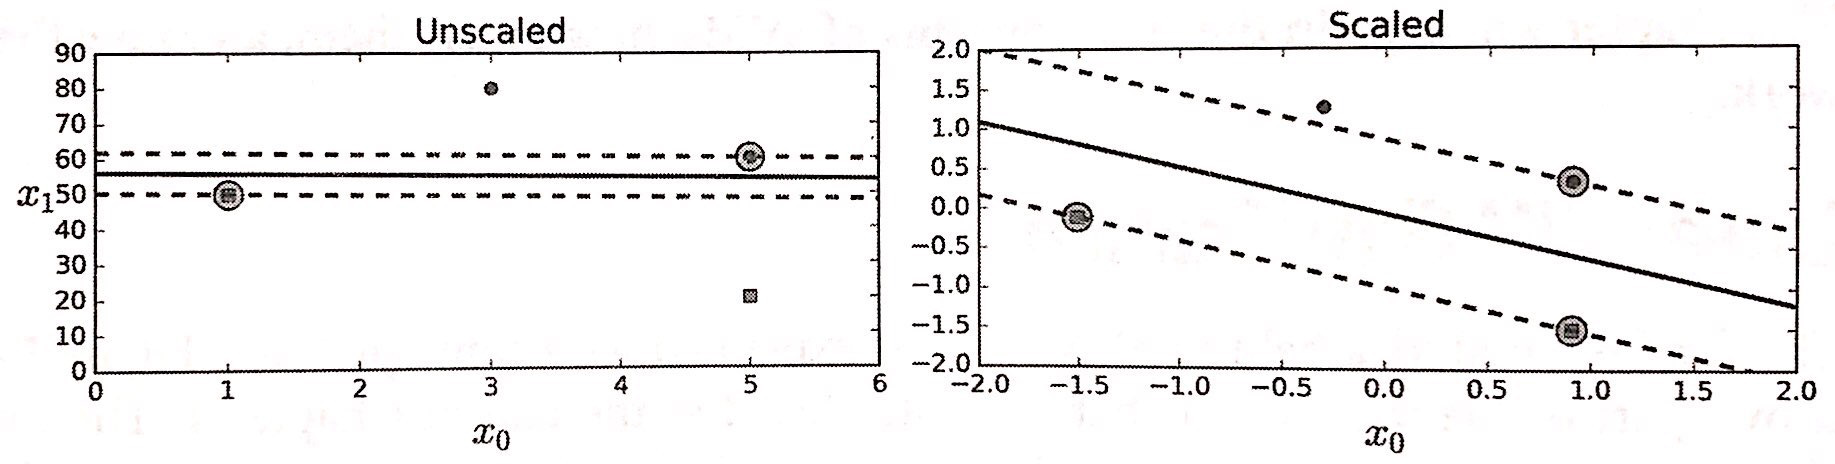
\includegraphics[scale=0.25]{Imagens/smv_escala.png}
    \caption{Sensibilidade com a escala dos dados \cite{Geron:2017}}
    \label{fig:svm-escala}
\end{figure}
